% ===== Part D: 4. 결합 원천-채널 부호화 / 5. 미해결 문제 / 6. 결론 (원문 31–37쪽) =====
\section{결합 원천-채널 부호화}

먼저 JSCC의 시스템 모형을 그림~6에 나타냈다. 부호기의 입력과 복호기의 출력은 길이 $k$인 벡터 $S^k$와 $Z^k$이다. 길이 $n$인 벡터 $X^n$과 $Y^n$은 각각 잡음 채널의 입력과 출력이다. JSCC의 부호율은 $\frac{k}{n}$으로 정의한다. 점근 영역에서 초과 왜곡 확률을 0으로 보내면, 달성 가능한 최대 JSCC 부호율은 $\frac{C}{R(d)}$이다. 여기서 $C$는 \emph{채널 용량}이고, $R(d)$는 미리 정한 평균 왜곡 제약 $d$ 아래의 \emph{율-왜곡 함수}이다. 이것이 [75]와 [66]의 원천-채널 분리 정리가 주는 고전적 결과이다. 다시 말해 점근 영역에서는 최적의 원천 부호와 채널 부호를 따로 설계한 뒤 이어 붙이기만 해도 점근적 근본 한계에 도달한다. 그러나 비점근 영역에서는 SSCC가 매우 느슨한 비점근 한계밖에 주지 못한다. 반면 JSCC 설계는 유한 부호 길이에서 상당한 이득을 낸다 [12]. 이는 두 설계 방식의 이론적 한계가 서로 다르며, 유한 부호 길이 영역에서 연구가 더 필요하다는 뜻이다.

Csiszár [55]는 JSCC의 오류 지수가 SSCC의 오류 지수보다 크다는 것을 증명했다. 평균 왜곡 기준 아래의 이산 원천-채널 쌍에 대해서는 Pilc [124, 56]가, 평균 제곱 오차 제약 아래에서 가우스 원천을 이산 채널로 전송하는 문제에 대해서는 Wyner [125, 57]가 비점근 한계를 얻었다. Csiszár는 [58]에서 그래프 이론적 JSCC 모형의 비점근 근본 한계도 유도했다. 거의 무손실인 JSCC 설정에서는 Campo 등 [126]이 유한 부호 길이 무작위 부호화 한계를 여럿 제시했다. 이어서 Wang 등 [59]은 원천과 채널의 알파벳이 유한한 경우에 JSCC의 분산도를 구했다. 끝으로 Kostina 등 [12]은 JSCC에 대한 새로운 일반적 달성 가능성 한계와 역 한계를 유도하고, 가우스 근사를 분석했으며, 여러 경우에 대한 결과를 얻었다. 이하에서는 JSCC의 근본 한계에 관한 주요 결과와 그 바탕에 있는 기본 아이디어를 살펴본다. 이어서 SSCC와 JSCC를 비교하며 유한 부호 길이에서 드러나는 성능 차이를 짚고, 실용 시스템을 위한 JSCC의 최근 진전을 요약하며 마무리한다.

\begin{figure}[t]
\centering
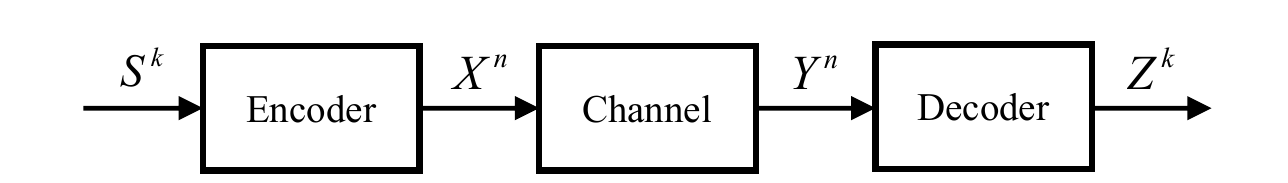
\includegraphics[width=0.85\linewidth]{fig/fig6.png}
\caption{결합 원천-채널 부호화의 시스템 모형.}
\end{figure}

\paragraph{1) 역 한계}
한편으로는 정보 확률변수를 바탕으로 일반적인 역 한계를 유도할 수 있다. 구체적으로, 상대 정보(relative information) $\iinf_{Y|X\|\bar{Y}}(x;y)=\log\frac{dP_{Y|X=x}}{dP_{\bar{Y}}}(y)$와 식~(8)의 $\dd$-기울인 정보 $\ttl_S(S,d)$의 차를 생각하면, 확률 $\P\bigl[\ttl_S(S,d)-\iinf_{Y|X\|\bar{Y}}(X;Y)\ge\gamma\bigr]$와 항 $e^{-\gamma}$의 차이가 초과 왜곡 확률 $\epsilon$을 넘지 않음을 보일 수 있다.\onote{원문 표현 그대로 옮겼다. [12]의 해당 정리를 식으로 쓰면 $\epsilon\ge\P\bigl[\ttl_S(S,d)-\iinf_{Y|X\|\bar{Y}}(X;Y)\ge\gamma\bigr]-e^{-\gamma}$ 꼴(임의의 $\gamma>0$과 $P_{\bar{Y}}$에 대해, 상황에 따라 $\sup$/$\inf$를 취함)로, 차이의 절댓값이 아니라 한쪽 방향 부등식이다.} 이 결과는 채널 입력의 형이 서로 다른 경우로 더 확장할 수도 있다.\onote{원문 ``extended when different channel input types''는 문장이 불완전하다. 채널 입력의 형별로 나누어 얻는 확장 한계를 가리키는 것으로 보고 옮겼다.} 다만 경우에 따라 이 방법으로 얻은 한계는 다소 느슨해진다.

다른 한편으로, Csiszár [55]는 $M$개 기호의 집합에서 원소 $L$개짜리 목록을 내놓는 목록 복호기를 써서 JSCC의 역 한계를 얻었다. Kostina 등 [12]은 이 기법을 유한 알파벳 원천에서 추상 알파벳 원천으로 확장하고, 여기에 가설 검정을 결합해 더 강한 역 한계를 얻었다.

\paragraph{2) 달성 가능성 한계}
최적 SSCC의 성능을 JSCC의 비점근 한계로 삼는 것은 자연스러운 발상이다. 실용적인 SSCC 방법 하나는 서로 독립인 무작위 원천 부호와 무작위 채널 부호를 쓰는 것이며, 이로부터 JSCC에 대해 계산 가능한 유한 부호 길이 달성 가능성 한계를 얻는다. 이 접근은 유한 부호 길이에서 SSCC가 왜 최적이 아닌지에 대해 중요한 통찰을 준다. 먼저 SSCC가 어떻게 점근적 한계에 도달하는지 보자. 부호 길이가 큰 영역에서 최적 원천 부호기의 출력은 대략 $\exp(kR(d))$개의 메시지로 이루어진 집합 위에서 거의 균등하게 분포하며, 이 메시지들이 정해진 왜곡 $d$ 이내에서 대부분의 원천 출력을 덮는다. 채널 부호화 정리에 따르면, 최대 우도(ML, maximum-likelihood) 복호기를 갖춘 채널 부호로 최대 $M=\exp(kR(d))<\exp(nC)$개의 메시지를 신뢰성 있게 구별할 수 있다. 따라서 최적의 원천 부호와 채널 부호를 이어 붙이면, $d>D(nC/k)$인 한 전체 방식의 초과 왜곡 확률은 무시할 만큼 작아진다. 그러나 유한 부호 길이에서는 최적 원천 부호기가 만드는 분포가 균등 분포와 거리가 멀다. 그 결과, 메시지 확률이 고르지 않다는 점을 고려하지 않고 ML 복호기를 쓰는 분리 방식은 최적에 가까운 비점근 성능에 이르지 못한다.

\paragraph{3) 근사}
JSCC 부호율의 가우스 근사를 소개하기 전에 몇 가지 조건을 밝혀 둔다. 원천과 채널은 정상이고 무기억이며, 왜곡 기준은 분리 가능하고 왜곡은 유계이다. 채널에 비용 함수가 있다면 그 비용 함수도 분리 가능해야 한다. 이 조건 아래에서 최적 $(k,n,d,\epsilon)$ 부호의 매개변수는 다음을 만족한다.
\begin{equation}
nC(\beta)-kR(d)=\sqrt{nV(\beta)+k\mathcal{V}(d)}\,Q^{-1}(\epsilon)+\theta(n),
\tag{34}
\end{equation}
여기서 $\mathcal{V}(d)$는 원천 분산도, $V(\beta)$는 채널 분산도이고, $\beta$는 채널 입력 비용 제약이다. 나머지 항 $\theta(n)$에 대해서는, 채널 입력 $X^n$과 출력 $Y^n$이 유한 알파벳 $\mathcal{X}$와 $\mathcal{Y}$ 위에서 정의되고 채널 비용 제약이 없으면 다음이 성립한다.
\begin{equation}
-c\log n+O(1)\le\theta(n)\le C_0\log n+\log\log n+O(1),
\tag{35}
\end{equation}
여기서 $c=|\mathcal{X}|-\frac{1}{2}$이고 $C_0=\frac{1}{2}+\frac{\Var\left(J'_{Z^\star}(\mathsf{S},\lambda^\star)\right)}{\E\left[|J''_{Z^\star}(\mathsf{S},\lambda^\star)|\right]\log e}$이며, $\lambda^\star=-\mathbb{R}'_{S}(d)$이다. 가우스 채널의 경우에 대한 추가 결과는 [12, Theorem 10]을 참고하라.

SSCC 아래의 근사는 [11]의 채널 부호화 결과와 [10]의 손실 원천 부호화 결과를 결합해 다음과 같이 얻는다.
\begin{equation}
nC(\beta)-kR(d)\le\min_{\eta+\zeta\le\epsilon}\left[\sqrt{nV(\beta)}\,Q^{-1}(\eta)+\sqrt{k\mathcal{V}(d)}\,Q^{-1}(\zeta)\right]+O(\log n).
\tag{36}
\end{equation}
채널과 원천 가운데 하나라도(또는 둘 다) 분산도가 0이면, 분리 부호화로도 결합 설계와 같은 전체 분산도를 달성할 수 있다. 이런 경우에는 $\dd$-기울인 정보나 채널 정보 밀도가 거의 결정적(deterministic)이어서, 최적 결합 원천-채널 부호가 이 확률적 양의 변동을 온전히 고려할 필요가 없기 때문이다.

\paragraph{4) SSCC와 JSCC의 비교}
식~(34)의 JSCC 근사와 식~(36)의 SSCC 근사를 비교하면, SSCC가 분리 설계 때문에 유한 부호 길이에서 성능을 잃는 이유를 더 직관적이고 간명하게 설명할 수 있다. 먼저 $k$와 $n$이 커질 때 CLT에 따라 $\dd$-기울인 정보와 채널 정보 밀도가 어떻게 행동하는지 보자. 원천이 정상이고 무기억이므로, 정규화한 $\dd$-기울인 정보 $J=\frac{1}{n}\ttl_{S^k}(S^k,d)$는 평균이 $\frac{k}{n}R(d)$이고 분산이 $\frac{k}{n}\frac{\mathcal{V}(d)}{n}$인 가우스 분포로 다가간다. 마찬가지로 조건부 정규화 채널 정보 밀도 $I=\frac{1}{n}\iinf^\star_{X^n;Y^n}(x^n;Y^{n\star})$는, 용량 달성 분포 아래에서 전형적인 모든 $x^n$에 대해 평균이 $C(\beta)$이고 분산이 $\frac{1}{n}V(\beta)$인 가우스 분포로 다가간다. 효율적인 부호기는 거의 모든 원천 실현값에 대해 이런 입력을 고르고, 원천과 채널은 서로 독립이다. 따라서 차 $I-J$ 역시 평균이 $C(\beta)-\frac{k}{n}R(d)$이고 분산이 $\frac{1}{n}\bigl(\frac{k}{n}\mathcal{V}(d)+V(\beta)\bigr)$인 가우스 분포에 가깝다.

JSCC에서는 식~(34)가 보여 주듯이, 채널 정보 밀도 $I$가 원천의 $\dd$-기울인 정보 $J$보다 클 때, 곧 사건 $\{I>J\}$가 일어날 때, 그리고 그때에만 원천을 왜곡 $d$ 이내로 복원할 수 있다. 반면 SSCC에서는 식~(36)이 보여 주듯이, 쌍 $(I,J)$가 두 반평면 $\{I>r\}$과 $\{J<r\}$의 교집합에 들어갈 때에만 높은 확률로 복원에 성공한다. 여기서 $r=\frac{\log M}{n}$은 원천 부호 블록과 채널 부호 블록 사이에 놓인 무잡음 채널의 용량을 나타낸다. 사건 $\{I>r\}\cap\{J<r\}$은 $\{I>J\}$의 진부분집합이므로, 분리 부호화 설계에서는 성능 손실이 생긴다.

\paragraph{5) JSCC의 최근 진전}
최근 연구는 실용적인 유한 부호 길이 통신 시스템에서 JSCC가 지닌 잠재력을 부각해 왔다. 과업 지향 JSCC 전략은 주어진 과업에 가장 관련 있는 정보만 전송하려 하며, 이는 저지연·대역폭 제약 환경에서 특히 유리하다 [60]. 딥러닝 기반 JSCC 방식은 유한 길이 원천 수열을 압축과 채널 부호화를 따로 거치지 않고 채널 입력으로 곧바로 사상할 수 있음을 보였다. 이런 방식은 채널 조건이 변해도 성능이 완만하게 저하되며, 짧은 부호 길이의 분리 기반 설계에서 흔히 나타나는 절벽 효과를 피한다 [61]. 더 나아가 JSCC에 채널 출력 되먹임을 도입하면 종단 간 복원 품질을 크게 높이고 전송 지연을 줄일 수 있다. 이는 유한 부호 길이 영역에서 현대 JSCC 기법이 지닌 구체적 이점을 보여 준다 [62].

\section{미해결 문제}

유한 부호 길이 정보이론에 많은 기여가 있었지만, 이 주제는 더 넓은 범위의 시나리오와 요구 조건에서 더 탐구되어야 한다. 이하에서는 이러한 미해결 문제와 향후 연구 방향 몇 가지를 자세히 논한다.

\subsection{촘촘하면서 해석적으로 다루기 쉬운 비점근 결과}

높은 정밀도와 해석적 다루기 쉬움을 함께 추구하는 일은 비점근 정보이론의 핵심 목표로 남아 있다. 기존 연구가 수많은 유한 부호 길이 한계와 근사를 유도했지만, 어떤 경우에는 엄밀한 정확도와 해석적 다루기 쉬움을 동시에 얻는 데 여전히 중대한 간극이 있다.

최근 [110]은 채널 부호화에서 중편차 영역의 3차 근사가 초단(超短) 부호 길이(예: $n=100$)와 극히 낮은 오류 확률(예: $10^{-10}$)에서도 놀라울 만큼 정확함을 보였다. 그러나 율-왜곡 문제에 대해서는 이에 상응하는 고차 근사가 아직 연구되지 않았으며, 이는 유망한 향후 연구 방향이다.

또한 대규모 무작위 접속에 필요한 최소 비트당 에너지에 대해, 수신 안테나가 하나인 페이딩 채널에서는 [49]가, MIMO 페이딩 채널에서는 [52, 53]이 비점근 달성 가능성 한계와 역 한계를 유도했다. 그러나 이 결과에는 복잡한 행렬 연산과 수치 최적화가 들어 있어 계산 부담이 크다. 따라서 해석적 촘촘함을 유지하면서도 복잡도가 낮은 비점근 한계가 필요하다. 아울러 계산 과정에 인공지능(AI, artificial intelligence) 기술 [127, 128]을 도입해 효율을 높이는 것도 흥미로운 방향이다.

\subsection{더 일반적인 시나리오의 비점근 결과}

단일 GMS의 경우, 율-왜곡 문제와 점진적 정밀화 문제의 2차 근사는 확립되었지만 다중 단말 손실 원천 부호화의 근본 한계는 여전히 미해결이다. 특히 GMS에 대한 Kaspi 문제의 비점근 달성 가능성 한계를 유도하는 일은 결코 간단하지 않다. 다중 기술(multiple descriptions) 문제에서는 GMS의 율-왜곡 영역이 확립되었지만 [129], 비점근 한계와 2차 근사를 유도하려면 새로운 기법이 필요하다.

채널 부호화에 관한 기존 비점근 결과도 더 일반적인 시나리오로 확장될 것으로 기대된다. 예를 들어 셀프리 대규모 MIMO는 넓어진 서비스 영역에서 많은 사용자를 지원하는 첨단 기법으로 제안되었다. 그러나 이러한 분산 안테나 시스템에서 채널 부호화의 유한 부호 길이 근본 한계는 아직 연구되지 않았다. 또한 기존 결과는 대부분 가우스 채널과 i.i.d.\ 페이딩 채널에 집중되어 있으며, 상관된 채널의 근본 한계는 여전히 미해결이다.

다중 원천, 페이딩 채널, 다중 수신 안테나처럼 더 넓은 부류의 원천과 채널에 대해 JSCC의 유한 부호 길이 근본 한계를 찾는 일은 매우 중요하며, 앞으로 다룰 만한 흥미로운 주제이다. 또한 의미 정보를 도입하는 것도 유망한 향후 연구 방향이다 [130, 131].

\subsection{효율적인 실용 방식 설계}

비점근 한계와 근사는 실용 통신 방식의 성능을 평가하는 이론적 기준점 역할을 한다. 기존 방식은 경우에 따라 이론적 결과와 상당한 격차를 보인다. 따라서 계산상 실현 가능성을 유지하면서 이론적 한계에 더 가까운 실용 방식을 개발하는 일이 꼭 필요하며, 이는 앞으로의 흥미로운 주제이다. 이 격차를 메우는 데 성공한다면, 새롭게 떠오르는 6G 사용 사례에서 지연에 민감한 응용을 지원하는 데 큰 의미가 있을 것이다.

\section{결론}

고전적인 점근 정보이론은 무한한 부호 길이와 페이로드 크기, 0으로 사라지는 오류 확률 같은 이상적인 가정에 기대고 있다. 그래서 지연에 민감한 실제 통신 시스템의 근본 한계를 규명하는 데에는 한계가 있다. 이런 이유로 저자들은 엄밀한 비점근 틀을 탐구하게 되었다. 이 작업에는 유한 부호 길이 영역의 난제를 풀 새로운 분석 도구와 기법이 필요하다. 이 논문에서는 비점근 근본 한계에 관한 최근 진전을 체계적으로 검토했다. 구체적으로, 정보이론적 비점근 근본 한계에 대한 다양한 비점근 달성 가능성 한계, 역 한계, 근사를 각 결과의 바탕에 있는 핵심 아이디어와 함께 제시했다. 먼저 원천 부호화의 기초 결과에서 출발해, P2P와 다중 단말 경우의 무손실 압축과 손실 압축을 모두 엄밀하게 분석했다. 이 과정에서 무기억 원천 모형과 기억이 있는 원천 모형을 아우르고, 원천 분포를 완전히 아는 경우와 통계적으로 불일치하는 경우를 모두 다루었다. 채널 부호화에 대해서는 P2P 시스템에서 데이터율, 오류 확률, 부호 길이 사이의 상충 관계에 관한 유한 부호 길이 결과를 논하고, 이어서 다중 접속 채널과 새로 떠오르는 대규모 접속 채널의 최근 진전을 다루었다. 나아가 JSCC의 비점근 결과를 제시했다. JSCC는 유한 부호 길이에서 분리 방식보다 상당한 성능 이점을 주는 것으로 나타났는데, 이는 고전적인 점근 정보이론의 결론과 다르다. 점근 지표에서 유한 부호 길이 정보이론으로 옮겨 가는 패러다임 전환 덕분에, 실제로 의미 있는 시나리오의 성능을 정확하게 규명할 수 있다. 또한 비점근 영역에서 근본 한계가 어떻게 행동하는지 알면 실용 방식을 평가할 수 있다. 실제로 실용 방식은 경우에 따라 이론적 결과와 큰 격차를 보였다. 끝으로 유한 부호 길이 정보이론의 미해결 과제 몇 가지를 논했다. 이 과제들은 미래 무선 통신 시스템을 위한 정보이론적 분석을 발전시키는 데 꼭 필요하다.
